\documentclass[tikz,border=5pt]{standalone}
\usepackage{tikz}
\usetikzlibrary{arrows.meta,patterns,decorations.pathreplacing}

% Atlas color palette
\definecolor{AtlasTeal}{HTML}{5BA4A4}
\definecolor{AtlasWarm}{HTML}{C17F59}
\definecolor{AtlasSage}{HTML}{7A9E7E}
\definecolor{AtlasTealLight}{HTML}{D4E8E8}

\begin{document}
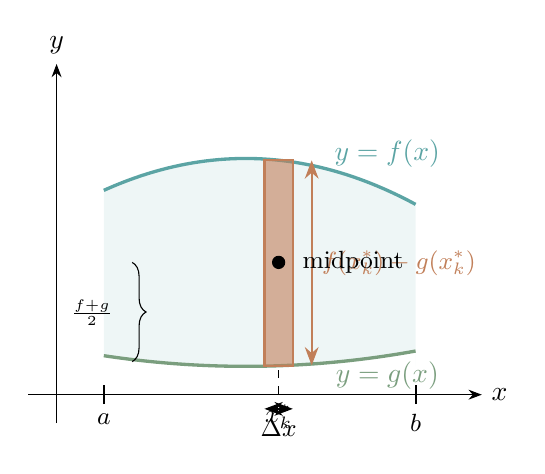
\begin{tikzpicture}[>=Stealth, scale=1.2]
    % Axes
    \draw[->] (-0.3,0) -- (4.5,0) node[right] {$x$};
    \draw[->] (0,-0.3) -- (0,3.5) node[above] {$y$};
    
    % Region fill (light)
    \fill[AtlasTealLight, opacity=0.4] 
        plot[domain=0.5:3.8, samples=50] (\x, {2.5 - 0.15*(\x-2)^2}) 
        -- (3.8,0.3) 
        -- plot[domain=3.8:0.5, samples=50] (\x, {0.3 + 0.05*(\x-2)^2}) 
        -- cycle;
    
    % Upper curve y = f(x)
    \draw[AtlasTeal, very thick, domain=0.5:3.8, samples=50] 
        plot (\x, {2.5 - 0.15*(\x-2)^2});
    \node[AtlasTeal, above] at (3.5, 2.3) {$y = f(x)$};
    
    % Lower curve y = g(x)
    \draw[AtlasSage, very thick, domain=0.5:3.8, samples=50] 
        plot (\x, {0.3 + 0.05*(\x-2)^2});
    \node[AtlasSage, below] at (3.5, 0.45) {$y = g(x)$};
    
    % Vertical strip (highlighted)
    \fill[AtlasWarm, opacity=0.6] 
        (2.2, {0.3 + 0.05*(2.2-2)^2}) rectangle (2.5, {2.5 - 0.15*(2.35-2)^2});
    \draw[AtlasWarm, thick] 
        (2.2, {0.3 + 0.05*(2.2-2)^2}) rectangle (2.5, {2.5 - 0.15*(2.35-2)^2});
    
    % Width label Δx
    \draw[<->, thick] (2.2, -0.15) -- node[below, font=\small] {$\Delta x$} (2.5, -0.15);
    
    % Height label
    \draw[<->, thick, AtlasWarm] (2.7, 0.31) -- 
        node[right, font=\small] {$f(x_k^*) - g(x_k^*)$} (2.7, 2.48);
    
    % Midpoint marker
    \fill[black] (2.35, 1.4) circle (2pt);
    \node[right, font=\small] at (2.5, 1.4) {midpoint};
    
    % x_k^* marker
    \draw[dashed] (2.35, 0) -- (2.35, 0.32);
    \node[below, font=\small] at (2.35, 0) {$x_k^*$};
    
    % Bounds a and b
    \draw[thick] (0.5, -0.1) -- (0.5, 0.1);
    \node[below, font=\small] at (0.5, -0.1) {$a$};
    \draw[thick] (3.8, -0.1) -- (3.8, 0.1);
    \node[below, font=\small] at (3.8, -0.1) {$b$};
    
    % Centroid formula annotation (y-midpoint)
    \draw[decorate, decoration={brace, amplitude=5pt, mirror}] 
        (0.8, 0.35) -- (0.8, 1.4);
    \node[left, font=\scriptsize] at (0.7, 0.87) {$\frac{f+g}{2}$};
\end{tikzpicture}
\end{document}
